\documentclass{article}
\usepackage[T1]{fontenc}
\usepackage{lmodern}
\usepackage{graphicx}
\usepackage{amsmath,amssymb}
\usepackage[a4paper,margin=2cm]{geometry}
\usepackage[absolute,overlay]{textpos}
\setlength{\TPHorizModule}{1mm}
\setlength{\TPVertModule}{1mm}
\usepackage[indonesian]{babel}
\usepackage{hyperref}
\setlength{\emergencystretch}{2em}
% unit: Halaman 12

\begin{document}

% === Halaman 12 (python/native) ===

12

Ancient Steganography

• Steganografi dengan media kepala budak.

 Ditulis oleh Herodatus  (485 – 525 BC), sejarawan Yunani pada tahun 440 BC di 

dalam buku: Histories of Herodatus). Kisah perang antara  kerajaan Persia dan 

rakyat Yunani.


 Herodatus menceritakan cara Histaiaeus mengirim pesan kepada Aristagoras of 

Miletus untuk melawan Persia. Caranya: Dipilih beberapa budak. Kepala budak 

dibotaki, ditulisi pesan dengan cara tato, rambut budak dibiarkan tumbuh, budak 

dikirim. Di tempat penerima kepala budak digunduli agar pesan bisa dibaca.

Herodatus

% deskripsi: gambar native xref 95
\noindent
\includegraphics[width=0.85\textwidth]{../../images/python/page_012_img_01.jpeg}

% deskripsi: gambar native xref 96
\noindent
\includegraphics[width=0.85\textwidth]{../../images/python/page_012_img_02.jpeg}

% deskripsi: gambar native xref 97
\noindent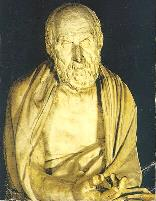
\includegraphics[width=0.85\textwidth]{../../images/python/page_012_img_03.jpeg}

\end{document}
